\documentclass[11pt, oneside]{article}   	% use "amsart" instead of "article" for AMSLaTeX format
\usepackage{geometry}                		% See geometry.pdf to learn the layout options. There are lots.
\geometry{letterpaper}                   		% ... or a4paper or a5paper or ... 
%\geometry{landscape}                		% Activate for for rotated page geometry
%\usepackage[parfill]{parskip}    		% Activate to begin paragraphs with an empty line rather than an indent
\usepackage{graphicx}				% Use pdf, png, jpg, or eps� with pdflatex; use eps in DVI mode
								% TeX will automatically convert eps --> pdf in pdflatex		
\usepackage{amssymb}
\usepackage{amsmath}
\usepackage{parskip}

\title{Shortest path}
%\author{The Author}
\date{}							% Activate to display a given date or no date

\graphicspath{{/Users/telliott_admin/Dropbox/Tex/png/}}

\begin{document}

\maketitle
%\section{}
% \subsection*{R code}
% \begin{lstlisting}  \end{lstlisting}
% \begin{center} 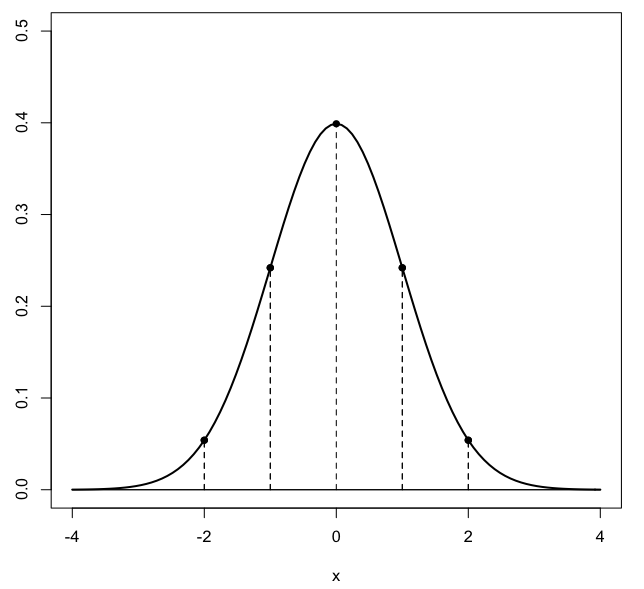
\includegraphics [scale=0.4] {gauss3.png} \end{center}
% \begin{bmatrix} a  &  b \\ c  &  d \end{bmatrix}
% \bigg |_

\Large
\noindent For this write-up our problem is shown in the figure below.  We have two points $P$ and $Q$, which might be, say, the origin and destination of a journey that must also go to the river (horizontal line at the top).  The point where we reach the river can be adjusted, and we seek the path that has the shortest overall distance.

\begin{center} 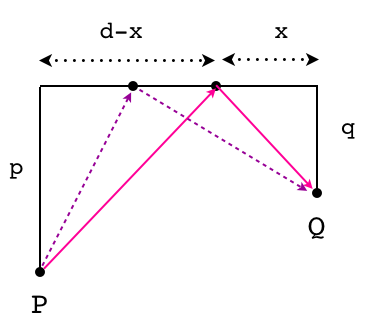
\includegraphics [scale=0.5] {short1.png} \end{center}

There is a hard way to do this problem, and an easy way.  The hard way involves a tiny bit of calculus (to do the minimization).  I'll show that one first.  

Depending on where we put the point on the river, we have a horizontal distance $x$ to that point from $Q$, and a horizontal distance $d-x$ to the same point from $P$.

The path consists of two parts, from $P$ to the river, and from the river back to $Q$.  That distance is
\[ \sqrt{p^2 + (d-x)^2} + \sqrt{q^2 + x^2} \]

We take the derivative with respect to $x$ and set that equal to $0$
\[- \frac{d-x}{\sqrt{p^2 + (d-x)^2}} +  \frac{x}{\sqrt{q^2 + x^2}} = 0\]
\[ \frac{x}{\sqrt{q^2 + x^2}} = \frac{(d-x)}{\sqrt{p^2 + (d-x)^2}} \]

Now it's just algebra.
\[ \frac{x^2}{q^2 + x^2} = \frac{(d-x)^2}{p^2 + (d-x)^2} \]

invert and simplify
\[ \frac{q^2}{x^2} + 1 = \frac{p^2}{(d-x)^2} + 1 \]

cancel $+1$ and take square roots
\[ \frac{q}{x} = \frac{p}{(d-x)} \]

The result is that the two triangles should be similar (since their sides are in proportion and they are both right triangles).  Another way to say it is that the angle where we come from $P$ to the river, and the angle by which we leave the river to $Q$ should be equal.

Now for the easy way.
\begin{center} 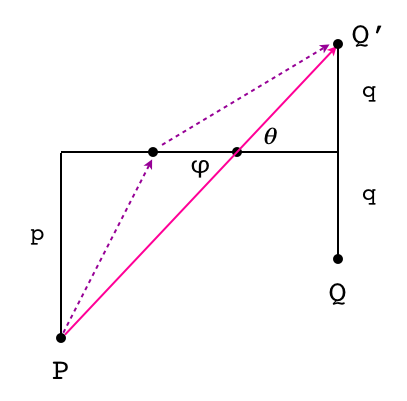
\includegraphics [scale=0.5] {short2.png} \end{center}
We draw a vertical up the same distance $q$ to point $Q'$---the mirror image of $Q$.  Minimizing the distance to $Q'$ is the same problem because it's exactly the same distance.

What's the shortest distance between two points?  A straight line from $P$ to $Q'$.  With a straight line then the two angles $\phi$ and $\theta$ are equal and the similarity of the triangles follows immmediately.

This is a famous result in physics.  It's true for light rays, that when you shine a light from $P$ at a mirror, the light rays arriving at $Q$ come by the shortest path.  The law about the angles being equal is called the "law of reflection" and it was known to Euclid.

Many pool players who know nothing about about Euclid know this result, and they use it all the time in making bank shots.

But this is only the beginning.  The general principle is called "least action."
\end{document}  